\documentclass[11pt,a4paper]{article}
\usepackage[margin=1in]{geometry}
\usepackage{enumitem}
\usepackage{amsmath}
\usepackage{amsfonts}
\usepackage{tikz}
\usetikzlibrary{arrows.meta, positioning, shapes.geometric}
\usepackage{listings}
\usepackage{xcolor}
\usepackage{graphicx}
\usepackage{fancyhdr}
\usepackage{titlesec}
\usepackage{booktabs}

% Clean styling
\titleformat{\section}{\large\bfseries}{\thesection}{1em}{}
\titleformat{\subsection}{\normalsize\bfseries}{\thesubsection}{1em}{}
\setlist[itemize]{noitemsep, topsep=0.5em}

\definecolor{codegreen}{rgb}{0,0.6,0}
\definecolor{codegray}{rgb}{0.5,0.5,0.5}

\lstdefinestyle{mystyle}{
    backgroundcolor=\color{white},   
    commentstyle=\color{codegreen},
    keywordstyle=\color{blue},
    numberstyle=\tiny\color{codegray},
    stringstyle=\color{codegray},
    basicstyle=\ttfamily\footnotesize,
    breakatwhitespace=false,         
    breaklines=true,                 
    captionpos=b,                    
    keepspaces=true,                 
    numbers=left,                    
    numbersep=5pt,                  
    showspaces=false,                
    showstringspaces=false,
    showtabs=false,                  
    tabsize=2
}
\lstset{style=mystyle}

\pagestyle{fancy}
\fancyhf{}
\rhead{DIGITAL LOGIC II (CPE 302)}
\lhead{Solutions}
\cfoot{\thepage}

\title{\textbf{DIGITAL LOGIC II (CPE 302) – SOLUTIONS}}
\author{}
\date{}

\begin{document}

\maketitle

\section*{QUESTION ONE}

\subsection*{(a) (i) Define registers.}
A register is a group of flip-flops (usually D-type or JK-type) used to store multiple bits of binary data. It acts as a high-speed temporary storage unit within a digital system, microprocessor, or computer, holding data, instructions, or addresses for processing.

\subsection*{(a) (ii) Highlight four ways by which the contents of registers can be operated on.}
\begin{enumerate}
    \item \textbf{Parallel Load}: All bits of the data are loaded simultaneously into the register on a single clock pulse.
    \item \textbf{Serial Shift (Left or Right)}: Data is shifted one bit at a time into or out of the register.
    \item \textbf{Clear (Reset)}: All bits within the register are set to logic 0.
    \item \textbf{Complement (Invert)}: The logic state of every bit is inverted (0 becomes 1, and 1 becomes 0).
\end{enumerate}

\subsection*{(b) (i) Examine the 74LS163 logic symbol, determine the conditions necessary to load the register in parallel.}
The 74LS163 is a 4-bit synchronous binary counter. The load operation is synchronous. To load data from the parallel inputs (A, B, C, D) into the register, the following conditions must be met:

\begin{itemize}
    \item The \textbf{LOAD} input must be set to LOW (Asserted).
    \item The \textbf{CLOCK} input must be in its active (rising) edge transition.
    \item Note: The enable inputs (ENP and ENT) must be HIGH to allow the counter to operate normally, though they are essentially disabled internally when LOAD is asserted.
\end{itemize}

\subsection*{(b) (ii) There are two distinct shift operations. Explain and illustrate with examples.}
The two distinct shift operations are Logical Shift and Arithmetic Shift.

\begin{enumerate}
    \item \textbf{Logical Shift}: The bits are shifted left or right, and the vacant bit positions are always filled with zeros.
       \begin{itemize}
           \item Example: 1101 logically shifted left by 1 becomes 1010.
       \end{itemize}
    \item \textbf{Arithmetic Shift}: This preserves the sign bit (most significant bit, MSB) for signed numbers. When shifting right, the vacant MSB position is filled with the existing sign bit. When shifting left, it is similar to logical shift but can indicate overflow.
       \begin{itemize}
           \item Example: 1101 (representing -3 in 2's complement) shifted right arithmetically by 1 becomes 1110 (representing -2).
       \end{itemize}
\end{enumerate}

\subsection*{(c) Determine the number of flip-flops needed.}
The counter must count up to 888 items. The number of flip-flops (N) required is determined by $2^N \geq$ Max Count.

\begin{itemize}
    \item $2^9 = 512$ (This is less than 888)
    \item $2^{10} = 1024$ (This is greater than 888)
\end{itemize}
Therefore, 10 flip-flops are required.

\section*{QUESTION TWO}

\subsection*{(a) (i) What is a counter? Discuss asynchronous counters with the aid of diagrams.}
A counter is a sequential digital circuit that progresses through a predetermined sequence of binary states upon the application of clock pulses. 

\textbf{Asynchronous (Ripple) Counters}: In these counters, the external clock signal is applied only to the first flip-flop (LSB). The output of each flip-flop serves as the clock signal for the next flip-flop in the chain.

\begin{center}
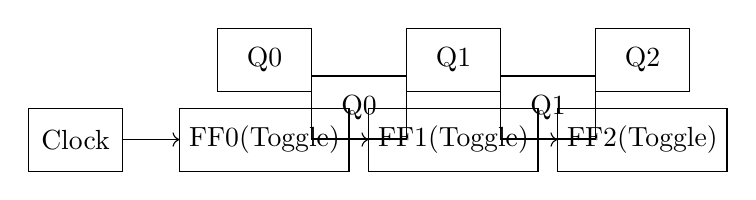
\begin{tikzpicture}[scale=0.8, every node/.style={draw, minimum width=1.2cm, minimum height=0.8cm}]
\node (clk) at (0,0) {Clock};
\node[draw, rectangle] (ff0) at (3,0) {FF0\\(Toggle)};
\node[draw, rectangle] (ff1) at (6,0) {FF1\\(Toggle)};
\node[draw, rectangle] (ff2) at (9,0) {FF2\\(Toggle)};
\draw[->] (clk) -- (ff0);
\draw[->] (ff0.east) -- node[above] {Q0} (ff1.west);
\draw[->] (ff1.east) -- node[above] {Q1} (ff2.west);
\node[above=0.2cm] at (ff0.north) {Q0};
\node[above=0.2cm] at (ff1.north) {Q1};
\node[above=0.2cm] at (ff2.north) {Q2};
\end{tikzpicture}
\end{center}

Because the clock ripples through the chain, the outputs do not change state simultaneously. This introduces propagation delay.

\subsection*{(a) (ii) The behavior of counters can be investigated in three different ways. Explain.}
\begin{enumerate}
    \item \textbf{Timing Diagram}: A graphical representation displaying the waveforms of the clock input and all flip-flop outputs alongside the time axis.
    \item \textbf{State Diagram}: A circle-and-arrow diagram illustrating the sequence of discrete states the counter cycles through.
    \item \textbf{State Table (Truth Table)}: A tabular listing showing the "Current State" and the corresponding "Next State" for every possible count.
\end{enumerate}

\subsection*{(b) (i) Compare serial data transfer to parallel data transfer.}
\begin{itemize}
    \item \textbf{Serial Data Transfer}: Data is transmitted one bit at a time along a single wire/line. It requires fewer physical interconnections but is slower. Example: USB communication.
    \item \textbf{Parallel Data Transfer}: All bits of a data word are transmitted simultaneously using multiple wires. It is much faster but requires more physical interconnections. Example: Internal system buses in computers.
\end{itemize}

\subsection*{(b) (ii) Determine:}
\begin{itemize}
    \item \textbf{I. The counter's MOD number}: 4 flip-flops $\rightarrow 2^4 = 16$. The MOD number is 16.
    \item \textbf{II. The frequency at the output of the last flip-flop}: 
          $f_{output} = \frac{f_{input}}{\text{MOD}} = \frac{1 \text{ MHz}}{16} = \mathbf{62.5 \text{ kHz}}$.
    \item \textbf{III. The range of counting states}: The range is from 0000 to 1111 (decimal 0 to 15).
    \item \textbf{IV. The counting state after 29 clock pulses}: 
          The counter wraps around every 16 pulses. $29 \mod 16 = 13$. The binary equivalent of 13 is 1101.
\end{itemize}

\subsection*{(c) Show how the 74LS293 can be connected to operate as a MOD 16 counter.}
The 74LS293 consists of a mod-2 counter and a mod-8 counter. To form a 4-bit mod-16 counter:

\begin{itemize}
    \item Connect the output of the first counter ($Q_A$) directly to the clock input of the second counter (Input B).
    \item Apply the external 10 kHz clock to Input 1 (the clock for the first counter).
    \item The resulting 4-bit outputs are $Q_A$, $Q_B$, $Q_C$, $Q_D$.
\end{itemize}

\section*{QUESTION THREE}

\subsection*{(a) (i) Define mode number and state the maximum binary number the counter can reach.}
The Mode Number (MOD) is the total number of distinct unique states that a counter cycles through before returning to its initial starting state. The maximum binary number a counter can reach is MOD - 1 (e.g., a MOD-16 counter reaches a maximum binary number of 15).

\subsection*{(a) (ii) Show how the 74LS293 can be connected to operate as a MOD 16 counter.}
(Same as Question 2(c))

\subsection*{(b) (i) Explain propagation delay in Asynchronous counters.}
Propagation delay is the time taken for a signal to pass through a logic gate or flip-flop. In an asynchronous (ripple) counter, the clock signal must propagate sequentially through all the flip-flops. Therefore, the total propagation delay is the sum of the individual propagation delays of every flip-flop in the chain. This limits the maximum operating frequency of the counter.

\subsection*{(b) (ii) How can a counter be modified to produce MOD numbers less than $2^N$. Explain using diagrams.}
A counter can be modified using feedback resetting. This involves decoding a specific state that represents the desired MOD number. When that state is reached, the output of a decoding gate (e.g., NAND) triggers the asynchronous Clear (CLR) inputs of all flip-flops, resetting the counter to 0000 immediately.

\begin{center}
\begin{tikzpicture}[scale=0.85]
\node[draw, rectangle, minimum width=1cm, minimum height=1cm] (ff3) at (0,2) {FF3};
\node[draw, rectangle, minimum width=1cm, minimum height=1cm] (ff2) at (2,2) {FF2};
\node[draw, rectangle, minimum width=1cm, minimum height=1cm] (ff1) at (4,2) {FF1};
\node[draw, rectangle, minimum width=1cm, minimum height=1cm] (ff0) at (6,2) {FF0};

\draw[->] (0,0) -- node[above] {CLK} (ff3.south);

\draw[->] (ff3.east) -- (ff2.west);
\draw[->] (ff2.east) -- (ff1.west);
\draw[->] (ff1.east) -- (ff0.west);

% NAND gate for reset
\node[draw, circle, minimum size=0.8cm] (nand) at (3,-1) {NAND};
\draw (ff3.south) -- (ff3.south |- nand.north);
\draw (ff1.south) -- (ff1.south |- nand.north);
\draw[->] (nand) -- ++(0,-0.5) -- ++(3,0) -- (ff3.south -| ++(3,0)) -- (ff3.south);
\draw[->] (nand.east) -- ++(1,0) -- ++(0,1) -- (ff0.south -| ++(1,0)) -- (ff0.south);

\node[above] at (ff3.north) {Q3};
\node[above] at (ff2.north) {Q2};
\node[above] at (ff1.north) {Q1};
\node[above] at (ff0.north) {Q0};
\end{tikzpicture}
\end{center}

For a MOD-10 counter, detect state 1010 using Q3 and Q1.

\subsection*{(c) Construct a MOD 14 Asynchronous counter. Determine the frequency.}
Use 4 flip-flops. Reset upon reaching state 14 (1110) using a NAND gate connected to Q3, Q2, Q1.

Frequency: $f_{output} = \frac{16 \text{ kHz}}{14} \approx \mathbf{1.14 \text{ kHz}}$.

\section*{QUESTION FOUR}

\subsection*{(a) (i) Explain synchronous counters. Hence, draw the excitation table of a typical flip-flop.}
In a Synchronous Counter, the external clock pulse is connected simultaneously to all the flip-flops. Because all flip-flops receive the clock at the exact same time, their outputs change state synchronously (in parallel), eliminating the cumulative propagation delay problem found in asynchronous counters.

\textbf{Excitation Table of a JK Flip-Flop:}

\begin{center}
\begin{tabular}{cccc}
\toprule
Current State (Q) & Next State (Q*) & J & K \\
\midrule
0 & 0 & 0 & X \\
0 & 1 & 1 & X \\
1 & 0 & X & 1 \\
1 & 1 & X & 0 \\
\bottomrule
\end{tabular}
\end{center}

\subsection*{(a) (ii) Explain frequency division multiplexing illustrating with example.}
Frequency Division Multiplexing (FDM) is a signal transmission technique where the total available transmission bandwidth is subdivided into a number of smaller, non-overlapping frequency bands. Each individual signal is modulated onto a different carrier frequency within these bands.

Example: Radio Broadcasting on different frequencies.

\section*{QUESTION FIVE}

\subsection*{(a) What is a decoder? Briefly describe two types of decoders.}
A decoder is a combinational logic circuit that converts binary information from n input lines to a maximum of $2^n$ unique output lines. Only one output line is active at a time.

\begin{itemize}
    \item \textbf{Binary Decoders} (e.g., 2-to-4, 3-to-8)
    \item \textbf{BCD-to-7-Segment Decoders}
\end{itemize}

\subsection*{(b) Design the logic for a 7446 BCD-to-7 segment decoder (Active Low).}
(Truth table and K-Map based logic expressions for segments a, b, etc.)

\subsection*{(c) A TSL (Tri-state Logic) circuit overcomes the shortcoming of a WIRED AND configuration. Explain.}
Tri-state Logic provides a High-Z state to avoid bus contention.

\subsection*{(d) (i) Control signals...}
1. RD (Read) 2. WR (Write) 3. CS/CE 4. Address Bus

\section*{QUESTION SIX}

\subsection*{(a) Define resolution...}
Resolution is the smallest step change in analog output. 

\[ K = \frac{V_{ref}}{2^n} \]

\subsection*{(b) (i) Differentiate between DAC and ADC using diagrams.}

\begin{center}
\textbf{DAC:}
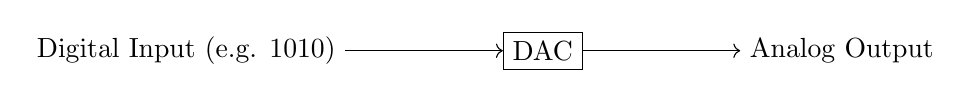
\begin{tikzpicture}
\node (in) {Digital Input (e.g. 1010)};
\node[right=2cm of in] (dac) [draw, rectangle] {DAC};
\node[right=2cm of dac] (out) {Analog Output};
\draw[->] (in) -- (dac);
\draw[->] (dac) -- (out);
\end{tikzpicture}

\textbf{ADC:}
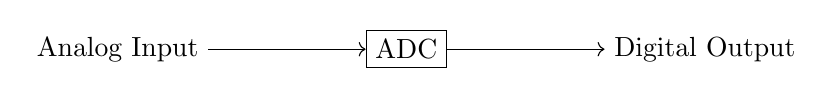
\begin{tikzpicture}
\node (in) {Analog Input};
\node[right=2cm of in] (adc) [draw, rectangle] {ADC};
\node[right=2cm of adc] (out) {Digital Output};
\draw[->] (in) -- (adc);
\draw[->] (adc) -- (out);
\end{tikzpicture}
\end{center}

\subsection*{(b) (ii)}
I. $R_{LSB} = 640\,\text{k}\Omega$

II. Resolution = $V_{ref}/64$

\section*{QUESTION SEVEN}

\subsection*{(a) Explain how a microcomputer bus work with the aid of diagrams.}
A microcomputer bus interconnects CPU, memory and I/O.

\begin{center}
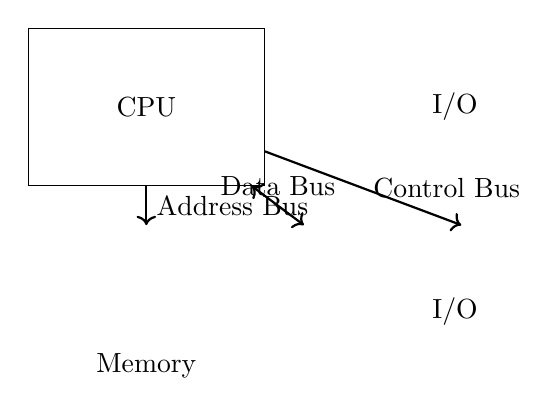
\begin{tikzpicture}[node distance=2cm]
\node[draw, rectangle, minimum width=3cm, minimum height=2cm] (cpu) {CPU};
\node[below=of cpu] (mem) {Memory};
\node[right=of cpu] (io1) {I/O};
\node[below=of io1] (io2) {I/O};

\draw[->, thick] (cpu) -- ++(0,-1.5) node[midway,right] {Address Bus};
\draw[<->, thick] (cpu) -- ++(2,-1.5) node[midway,above] {Data Bus};
\draw[->, thick] (cpu) -- ++(4,-1.5) node[midway,right] {Control Bus};
\end{tikzpicture}
\end{center}

\subsection*{(b) Design a synchronous counter...}
(Details as in original solution)

\subsection*{(c) With the aid of counter circuits differentiate between Johnson counter and ring counter.}

\textbf{Ring Counter}: $Q_{N-1} \to D_0$ (circulates single 1, MOD-N)

\textbf{Johnson Counter}: $\overline{Q_{N-1}} \to D_0$ (MOD-2N)

\subsection*{(d) A five-bit DAC...}
Output current for 1010 = \textbf{13.33 mA}

\section*{End of Solutions}
\end{document}